\section{The gamma factor, the Meixner law and the sine squared lemma}\label{ch:rz2}

In Section~\ref{ch:rz1} the gamma factor $G$ entered through the factorisation $\varphi=RG$ and its Thorin density $-\theta'(\sqrt t)/(2\pi\sqrt t)$, which changes sign at $t=\tau_0^2$. Its Weierstrass product writes this density as a renormalised series of Poisson kernels of widths $c_n=2n+\frac12$, and adding it to Proposition~\ref{rz:prop:theta} gives the formal Thorin measure of the reciprocal Xi function $R$ in Vere-Jones form. On the critical line $|G|^2$ is proportional to the density of a Meixner hypergeometric law, whose characteristic function is a GGC transform in the square of its variable and whose orthogonal polynomials satisfy a local Riemann Hypothesis. The sine squared lemma turns the L\'evy measure of $\log f$ into the Thorin measure of $f(0)/f(\sqs)$. It shows that after a stable tilt the reciprocals of $\zeta(\beta+\sqs)$, for $\beta>1$, and of the gamma factor are GGC transforms, and it shows how positivity is lost at the centre. Section~\ref{rz:sec:floor} follows the tilt of the gamma factor to the floor $e^{-c\sqs}R$ of the reciprocal Xi function.

\subsection{The gamma factor in Vere-Jones form}\label{rz:sec:gamma}

Recall from Section~\ref{rz:sec:intro} the constants $c_n=2n+\frac12$ for $n\ge0$ and $b=\frac12(\gamma_E+\log\pi)\approx0.860973$, where $\gamma_E$ is Euler's constant. With these constants the Weierstrass product writes $G$ as a product of GGC transforms whose Thorin densities are Poisson kernels, renormalised by stable factors.

\begin{theorem}\label{rz:thm:gamma}
For $s\in\cut$,
\[
G(s)=e^{-b\sqs}\prod_{n\ge0}\frac{e^{\sqs/(2n+2)}}{1+\sqs/c_n},
\]
and the Thorin measure of $G$ is
\[
U_G(dt)=\frac{1}{2\pi\sqrt t}\Bigl\{b+\sum_{n\ge0}\Bigl(\frac{c_n}{t+c_n^2}-\frac{1}{2n+2}\Bigr)\Bigr\}dt=-\frac{\theta'(\sqrt t)}{2\pi\sqrt t}\,dt .
\]
Each factor $(1+\sqs/\kappa)^{-1}$ is the Laplace transform of a GGC, with positive Thorin density $q_\kappa(t)=\dfrac{\kappa}{2\pi\sqrt t\,(t+\kappa^2)}$, a Poisson kernel in $\sqrt t$; each factor $e^{a\sqs}$ with $a>0$ has the negative Thorin density $-a/(2\pi\sqrt t)$.
\end{theorem}

\begin{proof}
Weierstrass gives $\log\Gamma(z_0+v)-\log\Gamma(z_0)=-\gamma_Ev-\log(1+v/z_0)+\sum_{n\ge1}\{v/n-\log(1+v/(n+z_0))\}$. Take $z_0=\frac14$, $v=\sqs/2$, note $v/(n+\frac14)=\sqs/c_n$, and shift the index of $v/n$. For $q_\kappa$: $\frac{d}{ds}\log(1+\sqs/\kappa)=\frac{1}{2\sqs(\sqs+\kappa)}$, and Lemma~\ref{rz:lem:inv} with $\sqrt{-t+i0}=i\sqrt t$ gives the density $\frac{\kappa}{2\pi\sqrt t(t+\kappa^2)}$. For $e^{a\sqs}$ use $\int_0^\infty\log(1+s/t)t^{-1/2}dt=2\pi\sqs$. To sum the Thorin densities of the factors, write the bracket with index $n$ in $U_G$ as $(\frac1{c_n}-\frac1{2n+2})-\frac{t}{c_n(t+c_n^2)}$: both parts are nonnegative, and over $n$ the first sums to a constant and the second to $O(\log(2+t))$, so Tonelli's theorem applies to each part against $\log(1+s/t)\frac{dt}{2\pi\sqrt t}$ for $s>0$, and analytic continuation extends the sum to $\cut$; the same split justifies the termwise integration against $e^{-tx}$ in Proposition~\ref{rz:prop:W0erfc}. The identification with $\theta'$ is the partial fraction series $\Re\psi(\frac14+\frac{i\tau}2)=-\gamma_E+\sum_{n\ge0}\{\frac1{n+1}-\frac{2c_n}{c_n^2+\tau^2}\}$.
\end{proof}

Formally, the gamma factor is thus a renormalised infinite convolution of GGC laws, and the renormalisation is the only source of negativity in its Thorin density. Write $X_\varphi$ and $X_R$ for random variables with Laplace transforms $\varphi$ and $R$; both laws exist and are infinitely divisible, by Theorem~\ref{rz:thm:id} and by Theorem~\ref{thm:ch12:idsd} \cite[Theorem A]{P26}. Write $Y_\kappa$ for the variable with $\E e^{-sY_\kappa}=\kappa/(\kappa+\sqs)$, which is $Y_\kappa=E_\kappa^2/(4\Gamma_{1/2})$ with $E_\kappa$ exponential of rate $\kappa$ and $\Gamma_{1/2}$ an independent gamma variable of shape $\frac12$, and $L_a$ for the positive stable variable of index $\frac12$ with $\E e^{-sL_a}=e^{-a\sqs}$. Theorem~\ref{rz:thm:gamma} and Proposition~\ref{rz:prop:rh} then say formally
\begin{equation}\label{rz:eq:decon}
X_\varphi\;\overset{d}{=}\;X_R+L_b+\sum_{n\ge0}\bigl(Y_{c_n}\ominus L_{1/(2n+2)}\bigr),
\end{equation}
where $A\ominus B$ stands for a formal variable whose Laplace transform is the quotient of those of $A$ and $B$. Each bracket has Thorin density $\frac{1}{2\pi\sqrt t}\{\frac{c_n}{t+c_n^2}-\frac1{2n+2}\}$, positive for $t<\frac32c_n$ and negative beyond. The sum of the $Y_{c_n}$ diverges almost surely because $\sum1/c_n=\infty$, and the stable deconvolutions are the compensators that make the product of the Laplace transforms converge.

Figure~\ref{rz:fig:UG} shows the Thorin density of $G$ against the first three kernels. In the variable $\tau=\sqrt t$ it is $-\theta'(\tau)/\pi$, evaluated from the digamma function, so nothing in it depends on a zero of $\zeta$. It changes sign at the point $\tau_0$ where $\theta$ attains its minimum, so the reciprocal $1/G$ has a Thorin density that is negative near the origin, and $1/G$ becomes a GGC only after the stable tilt of Theorem~\ref{rz:thm:gammaggc}.

\begin{figure}[htbp]
\centering
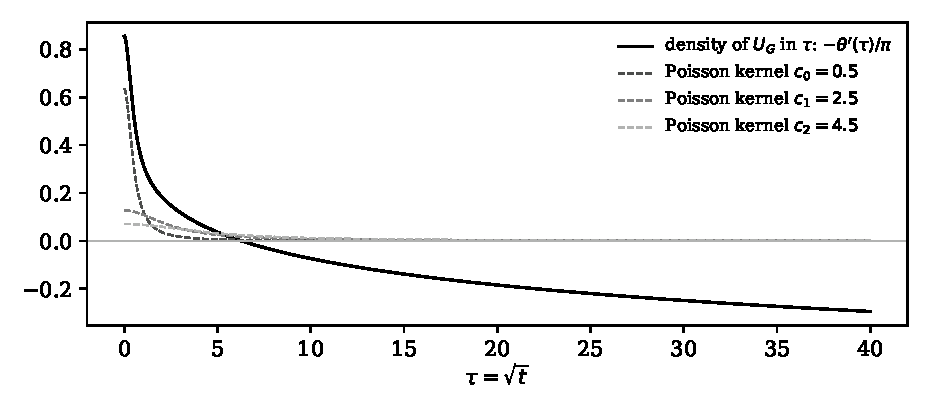
\includegraphics[width=0.9\textwidth]{rzfig/fig_UG.pdf}
\caption{The Thorin density of the gamma factor in the variable $\tau=\sqrt t$, namely $-\theta'(\tau)/\pi$, together with the first three Poisson kernels $c_n/(\pi(c_n^2+\tau^2))$ of Theorem~\ref{rz:thm:gamma}. The density is positive for $\tau<\tau_0\approx6.29$ and negative beyond, where the flat compensators outweigh the kernels.}
\label{rz:fig:UG}
\end{figure}

\begin{proposition}\label{rz:prop:W0erfc}
For $x>0$,
\[
W_0(x)=-\int e^{-tx}\,U_G(dt)=-\frac{b}{2\sqrt{\pi x}}+\sum_{n\ge0}\Bigl\{\frac{1}{(4n+4)\sqrt{\pi x}}-\frac12e^{c_n^2x}\operatorname{erfc}\bigl(c_n\sqrt x\bigr)\Bigr\}.
\]
\end{proposition}

\begin{proof}
$\int_0^\infty e^{-tx}q_\kappa(t)\,dt=\frac\kappa\pi\int_0^\infty\frac{e^{-xv^2}}{v^2+\kappa^2}dv=\frac12e^{\kappa^2x}\operatorname{erfc}(\kappa\sqrt x)$ and $\int_0^\infty e^{-tx}\frac{dt}{2\pi\sqrt t}=\frac{1}{2\sqrt{\pi x}}$.
\end{proof}

Both terms of the identity $W=w+W_0$ of \eqref{rz:eq:weil} are now explicit, and their sum is the heat trace over the zeros.

\begin{theorem}\label{rz:thm:RLVJ}
For every $x>0$, with absolutely convergent sums,
\begin{multline*}
W(x)=e^{x/4}+\sum_{N\ge2}B_N\,h_{\log N}(x)-\frac{b}{2\sqrt{\pi x}}\\
+\sum_{n\ge0}\Bigl\{\frac{1}{(4n+4)\sqrt{\pi x}}-\frac12e^{c_n^2x}\operatorname{erfc}\bigl(c_n\sqrt x\bigr)\Bigr\}.
\end{multline*}
Equivalently, $W(x)$ is the Laplace transform, taken term by term, of the formal series
\begin{multline*}
U_R=\delta_{-1/4}+\sum_{N\ge2}B_N\Bigl\{\sum_{k\ge0}\delta_{\sigma_k(\log N)}-\frac{\log N}{4\pi\sqrt t}\,dt\Bigr\}\\
-\frac{1}{2\pi\sqrt t}\Bigl\{b+\sum_{n\ge0}\Bigl(\frac{c_n}{t+c_n^2}-\frac1{2n+2}\Bigr)\Bigr\}dt ,
\end{multline*}
the formal Thorin measure of $R(s)=\xi(\frac12)/\xi(\frac12+\sqs)$. Under RH, $R$ is a GGC, and its Thorin measure $\sum_{\gamma>0}\delta_{\gamma^2}=dN(\sqrt t)$, where $N(T)$ counts the zeros with $0<\gamma\le T$, is a positive measure whose Laplace transform is also $W$.
\end{theorem}

\begin{proof}
$W=w+W_0$ by \eqref{rz:eq:weil}; substitute Proposition~\ref{rz:prop:theta} for $w$ and Proposition~\ref{rz:prop:W0erfc} for $W_0$. Term by term, $\delta_{-1/4}$ has Laplace transform $e^{x/4}$, the bracket with index $N$ has transform $h_{\log N}(x)$ by the definition of $h_\lambda$, and the last density is $-U_G$, whose transform is $W_0(x)$ by Proposition~\ref{rz:prop:W0erfc}. Under RH, Hadamard's product gives $R(s)=\prod_{\gamma>0}(1+s/\gamma^2)^{-1}$, as in the proof of Theorem~\ref{rz:thm:thorin}, and $W(x)=\sum_{\gamma>0}e^{-x\gamma^2}$ by Theorem~\ref{rz:thm:w}.
\end{proof}

The formula is the explicit formula for the heat trace in closed form: the polar term $e^{x/4}$, a sum over prime powers of the block theta functions $h_{\log N}$ weighted by the coefficients $B_N$ of Theorem~\ref{rz:thm:saw}, which Theorem~\ref{rz:thm:necklace} of Section~\ref{ch:rz3} expresses through necklace polynomials, and a sum of complementary error functions over the poles of the gamma factor. Each term is elementary and computable to high accuracy, and Table~\ref{rz:tab:num} checks the identity against the zero sum to twenty digits at $x=0.005$, $0.01$ and $0.03$.

In $U_R$ the pole gives an atom at $-\frac14$, off the half line $(0,\infty)$ that carries Thorin measures. The primes give lattices of sech atoms at $((2k+1)\pi/\log N)^2$, each compensated by its mean density. The gamma factor gives negative Poisson kernels of widths $c_n$ in the variable $\sqrt t$, with poles at $\sqrt t=\pm ic_n$, each compensated by a positive flat density. RH is the statement that the three groups combine into unit atoms at the $\gamma^2$ and nothing else. They combine only through Laplace transforms: every partial sum of $U_R$ carries the atom at $-\frac14$ and the Thorin measure $\sum_{\gamma>0}\delta_{\gamma^2}$ of $R$ under RH does not, so, like the series after Proposition~\ref{rz:prop:theta}, $U_R$ does not converge to that measure as a series of measures. By Theorem~\ref{rz:thm:crit}, $R$ has a Thorin type representation only if RH holds, since adding $U_G$ to its measure would give a measure $m$ as in condition (ii) there.

On the cut the gamma factor has modulus and phase
\[
G(-\tau^2+i0)=\frac{|\Gamma(\frac14+\frac{i\tau}2)|}{\Gamma(\frac14)}\,e^{i\theta(\tau)} .
\]
The phase is the Riemann Siegel theta function, and it is $-\pi$ times the distribution function of the Thorin measure: $U_G((0,\tau^2])=-\theta(\tau)/\pi$, since $\Im\log(1+s/t)=\pi$ for $t<\tau^2$ at $s=-\tau^2+i0$. The modulus is the logarithmic potential of the same measure,
\begin{equation}\label{rz:eq:pot}
\log\frac{|\Gamma(\frac14+\frac{i\tau}2)|}{\Gamma(\frac14)}=-\int\log\Bigl|1-\frac{\tau^2}{t}\Bigr|\,U_G(dt),
\end{equation}
the integral converging absolutely.

The square of the modulus is proportional to the density of a Meixner hypergeometric law, with parameter $a=\frac14$; Lai and Vere-Jones \cite{LVJ} study this family and its case $a=\frac12$, the hyperbolic secant law. Since $\int|\Gamma(a+ix)|^2e^{iux}dx=2\pi\Gamma(2a)(2\cosh\frac u2)^{-2a}$,
\begin{equation}\label{rz:eq:meixner}
p(\tau)=\frac{|\Gamma(\frac14+\frac{i\tau}2)|^2}{2^{3/2}\pi^{3/2}}\quad\text{is a probability density with}\quad\int p(\tau)e^{iv\tau}d\tau=\sech(v)^{1/2}.
\end{equation}
In this section $p$ denotes this Meixner density; the P\'olya density $\Phi/\Xi(0)$ of Section~\ref{ch:clock} does not occur. Since $\Xi(\tau)=-\frac12(\tau^2+\frac14)\pi^{-1/4}|\Gamma(\frac14+\frac{i\tau}2)|Z(\tau)$, with Hardy's function $Z(\tau)=e^{i\theta(\tau)}\zeta(\frac12+i\tau)$ of Section~\ref{ch:classical}, the Meixner density is the archimedean part of $\Xi^2$ on the critical line:
\[
\Xi(\tau)^2=\tfrac14\bigl(\tau^2+\tfrac14\bigr)^2\,2^{3/2}\pi\,p(\tau)\,Z(\tau)^2 .
\]
Lai and Vere-Jones call the Meixner hypergeometric distribution the odd man out; the characteristic function $\sech(v)^{1/2}$ of $p$ is a power of the kernel of Proposition~\ref{rz:prop:lvj}. We return to this law in Section~\ref{rz:sec:meixner}.

\subsection{From L\'evy to Thorin: the sine squared lemma}\label{rz:sec:sin2}

For a function of the form $f(0)/f(\sqs)$ we call $f$ its primal function. The sine squared lemma of \cite[Lemma 1]{P17v5} converts the L\'evy measure of $\log f$ into the Thorin measure of $f(0)/f(\sqs)$. The Vere-Jones representation produces such L\'evy measures, sums of atoms at the points $k\log N$, so the lemma applies to them. We state it in its original scaling and then in the coordinates of Section~\ref{rz:sec:intro}.

\begin{lemma}[{\cite[Lemma 1]{P17v5}}]\label{rz:lem:P1}
Suppose that for some measure $\mu$ on $(0,\infty)$ and some $\alpha$ with $\int_0^\infty(1\wedge x)e^{-\alpha x}\,\mu(dx)<\infty$,
\[
\log\frac{f(\alpha+s)}{f(\alpha)}-s\frac{f'(\alpha)}{f(\alpha)}=\int_0^\infty\bigl(e^{-sx}-1+sx\bigr)e^{-\alpha x}\,\frac{\mu(dx)}x,\qquad s\ge0 .
\]
Then, for $s\ge0$,
\[
\log\frac{f(\alpha)}{f(\alpha+s)}+s\frac{f'(\alpha)}{f(\alpha)}=-\int_0^\infty\bigl(1-e^{-\frac12s^2t}\bigr)\frac{\nu_\alpha(t)}t\,dt,
\]
\[
\nu_\alpha(t)=\frac{1}{\sqrt{2\pi}}\int_0^\infty e^{-tz}\Bigl\{\int_0^\infty2\sin^2\bigl(x\sqrt{z/2}\bigr)e^{-\alpha x}\,\mu(dx)\Bigr\}\frac{dz}{\sqrt{\pi z}} .
\]
The map $\mu\mapsto\nu_\alpha$ is linear and positivity preserving.
\end{lemma}

In these coordinates, with $s=u^2$ and $u=\sqs$, the lemma reads as follows. We include the proof by subordination, because its two stages, a L\'evy density in $s$ followed by a Thorin density, reappear in Section~\ref{rz:sec:floor}.

\begin{lemma}[Lemma~\ref{rz:lem:P1} in the scaling $s=u^2$]\label{rz:lem:sin2}
Let $\tilde\mu$ be a signed measure on $(0,\infty)$ with $\int(1\wedge x)|\tilde\mu|(dx)<\infty$, and suppose
\[
\log\frac{f(u)}{f(0)}-u\frac{f'(0)}{f(0)}=\int_0^\infty\bigl(e^{-ux}-1+ux\bigr)\frac{\tilde\mu(dx)}x,\qquad u\ge0 .
\]
Then for $s\in\cut$
\begin{gather*}
\log\frac{f(0)}{f(\sqs)}+\sqs\,\frac{f'(0)}{f(0)}=-\int_0^\infty\log\Bigl(1+\frac st\Bigr)U(t)\,dt,\\
U(t)=\frac{1}{2\pi\sqrt t}\int_0^\infty2\sin^2\Bigl(\frac{x\sqrt t}2\Bigr)\tilde\mu(dx).
\end{gather*}
If $\tilde\mu\ge0$ then $U\ge0$, and $s\mapsto f(0)e^{\sqs f'(0)/f(0)}/f(\sqs)$ is the Laplace transform of a GGC. Since $\sqs=\int\log(1+s/t)\,\frac{dt}{2\pi\sqrt t}$, the Thorin measure of $f(0)/f(\sqs)$ itself is $U(t)\,dt+\frac{f'(0)}{f(0)}\frac{dt}{2\pi\sqrt t}$.
\end{lemma}

\begin{proof}
Subordination by the first passage law \eqref{rz:eq:levy} gives, for $x,u>0$,
\[
e^{-ux}-1+ux=\int_0^\infty\bigl(1-e^{-u^2y}\bigr)\bigl(1-e^{-x^2/4y}\bigr)\frac{x}{\sqrt{4\pi y^3}}\,dy,
\]
because $\int_0^\infty(1-e^{-u^2y})\frac{x}{\sqrt{4\pi y^3}}dy=ux$. Integrating against $\tilde\mu(dx)/x$ gives a L\'evy form in $s=u^2$ with L\'evy density $k(y)/y$, where $k(y)=(4\pi y)^{-1/2}\int(1-e^{-x^2/4y})\tilde\mu(dx)$ is the canonical function. Finally $(1-e^{-x^2/4y})/\sqrt y=\int_0^\infty e^{-yt}\{1-\cos(x\sqrt t)\}\frac{dt}{\sqrt{\pi t}}$, so $k(y)=\int e^{-yt}U(t)dt$, and Frullani turns $\int(1-e^{-sy})k(y)\frac{dy}y$ into $\int\log(1+s/t)U(t)dt$. All kernels in these steps are nonnegative, so by Tonelli's theorem the steps hold with $|\tilde\mu|$ in place of $\tilde\mu$, and there every integral is finite, since $0\le(e^{-ux}-1+ux)/x\le\min(\frac{u^2x}2,u)$ and $\int(1\wedge x)|\tilde\mu|(dx)<\infty$; this justifies each interchange for the signed $\tilde\mu$. The analytic continuation to $\cut$ is immediate.
\end{proof}

Lemma~\ref{rz:lem:sin2} is \eqref{eq:sin2} of Section~\ref{ch:clock} integrated against $\tilde\mu(dx)/x$; the letters $s$ and $u$ are exchanged between the two sections. We call $\tilde\mu$ the primal L\'evy measure of $f(0)/f(\sqs)$. Positivity comes from the kernel. The signed cosine density that Lemma~\ref{rz:lem:inv} produces for a single exponential in an exponent (Section~\ref{rz:sec:prelim}) is $-\cos=2\sin^2-1$, and Lemma~\ref{rz:lem:sin2} separates it into the positive part $2\sin^2$ and a flat part $-1$, which is absorbed into the linear tilt $u\,f'(0)/f(0)$, a stable law of index $\frac12$.

\subsubsection{Zeta to the right of the line, the Vere-Jones blocks and the centre}

Where the primal L\'evy measure is positive the lemma applies directly. The first such case is $\zeta$ to the right of $\Re z=1$.

\begin{proposition}\label{rz:prop:zetaright}
For $\beta>1$ put $\tilde\mu_\beta=\sum_{n\ge2}\Lambda(n)n^{-\beta}\delta_{\log n}$. Then
\[
\frac{\zeta(\beta)}{\zeta(\beta+\sqs)}\,e^{\sqs\,\zeta'(\beta)/\zeta(\beta)}
=\exp\Bigl(-\int_0^\infty\log\Bigl(1+\frac st\Bigr)U_\beta(t)\,dt\Bigr),
\]
\[
U_\beta(t)=\frac{1}{2\pi\sqrt t}\sum_{n\ge2}\frac{\Lambda(n)}{n^\beta}\,2\sin^2\Bigl(\frac{\sqrt t\log n}2\Bigr)\ge0,
\]
so the left side is the Laplace transform of a GGC. Adding the tilt, the Thorin measure of $\zeta(\beta)/\zeta(\beta+\sqs)$ is $-\frac{1}{2\pi\sqrt t}\sum\Lambda(n)n^{-\beta}\cos(\sqrt t\log n)\,dt$, which is the Euler product density \eqref{rz:eq:formal} at $\beta$ in place of $\frac12$.
\end{proposition}

\begin{proof}
$\log\zeta(\beta+u)=\sum\Lambda(n)n^{-\beta}e^{-u\log n}/\log n$, so the hypothesis of Lemma~\ref{rz:lem:sin2} holds with $\tilde\mu_\beta$, which has finite mass for $\beta>1$.
\end{proof}

The tilt is needed: without it the Thorin density
\[
-\frac{1}{2\pi\sqrt t}\sum\Lambda(n)n^{-\beta}\cos(\sqrt t\log n)
\]
is negative near $t=0$. For $\xi$ no tilt is needed, since $s\mapsto\xi(\alpha)/\xi(\alpha+\sqs)$ is a GGC transform for every $\alpha\ge1$ (Theorem~\ref{thm:poisson}); at $\alpha=1$, Section~\ref{ch:basepoint} obtains its Thorin density from a L\'evy form of $\log\xi(1+u)$ by the same lemma. As $\beta\downarrow1$ the mass $\sum\Lambda(n)n^{-\beta}$ diverges, and at $\beta=\frac12$, where the pole and the gamma factor also enter, the lemma cannot be applied as it stands. The rest of this chapter and Chapter~\ref{chap:rzid} try to extend the case $\beta>1$ towards the critical line.

The Vere-Jones blocks have signed primal L\'evy measures, yet the lemma still gives positive Thorin densities. Apply it to one block $f_\lambda(u)=1+e^{-\lambda u}$ of Theorem~\ref{rz:thm:saw}, shifted by $\alpha>0$. Since $\log(1+e^{-\lambda(\alpha+u)})=\sum_k(-1)^{k+1}q^ke^{-k\lambda u}/k$ with $q=e^{-\lambda\alpha}$, the primal L\'evy measure is the alternating lattice $\tilde\mu_{\lambda,\alpha}=\lambda\sum_{k\ge1}(-1)^{k+1}q^k\delta_{k\lambda}$.

\begin{proposition}\label{rz:prop:block}
For $\alpha>0$ the sine squared transform of $\tilde\mu_{\lambda,\alpha}$ is positive:
\[
U_{\lambda,\alpha}(t)=\frac{\lambda}{2\pi\sqrt t}\,\frac{q(1-q)\bigl(1-\cos\lambda\sqrt t\bigr)}{(1+q)\bigl(1+2q\cos\lambda\sqrt t+q^2\bigr)}\ge0,
\]
so $\frac{1+e^{-\lambda\alpha}}{1+e^{-\lambda(\alpha+\sqs)}}\,e^{-\sqs\lambda q/(1+q)}$ is the Laplace transform of a GGC. As $\alpha\downarrow0$, $U_{\lambda,\alpha}(t)\,dt\to\sum_{k\ge0}\delta_{\sigma_k(\lambda)}$ vaguely, the tilt density tends to $-\frac{\lambda}{4\pi\sqrt t}$, and the Thorin measure of $2/(1+e^{-\lambda\sqs})$ is recovered as $\sum_k\delta_{\sigma_k(\lambda)}-\frac{\lambda}{4\pi\sqrt t}dt=-U_\lambda$, the sawtooth measure of Lemma~\ref{rz:lem:saw}.
\end{proposition}

\begin{proof}
$\sum_k(-1)^{k+1}q^k=\frac q{1+q}$ and $\sum_k(-1)^{k+1}q^k\cos k\omega=\frac{q\cos\omega+q^2}{1+2q\cos\omega+q^2}$; their difference is $\frac{q(1-q)(1-\cos\omega)}{(1+q)(1+2q\cos\omega+q^2)}\ge0$. As $q\uparrow1$ this is a Poisson kernel in $\omega=\lambda\sqrt t$ concentrating at $\omega=(2k+1)\pi$ with mass $\pi$ per period, which becomes $\sum_k\delta_{\sigma_k(\lambda)}$ after the change of variable. The tilt is $f'(\alpha)/f(\alpha)=-\lambda q/(1+q)\to-\lambda/2$.
\end{proof}

The sine squared image of each block is a Poisson kernel in $\sqrt t$ for $\alpha>0$ and the sech lattice at $\alpha=0$, so the negative part of the sawtooth measure is entirely the tilt. Summing the blocks with the weights $B_N$ gives $\log\zeta(\frac12+\alpha+\sqs)$, and the sum of Thorin densities $\sum_NB_NU_{\log N,\alpha}$ converges absolutely for $\alpha>\frac12$, where it equals $U_{1/2+\alpha}$ of Proposition~\ref{rz:prop:zetaright}. Positivity is then visible termwise in the prime form. It is not visible blockwise in the Vere-Jones form, because infinitely many weights are negative: $B_{p^3}=\frac13(p^{-3/2}-p^{-1/2})<0$ for every prime $p$, and Proposition~\ref{rz:prop:signs} of Section~\ref{ch:rz3} gives infinitely many more.

At $\beta=\frac12$ the prime L\'evy measure $\tilde\mu_{1/2}=\sum\Lambda(n)n^{-1/2}\delta_{\log n}$ has infinite mass, and both the image and the tilt in Lemma~\ref{rz:lem:sin2} diverge: the positive sine squared image has density of order $\frac{1}{2\pi\sqrt t}\sum\Lambda(n)n^{-1/2}=\infty$, and the tilt $\zeta'/\zeta(\frac12+0)$ is $-\infty$ along the Dirichlet series. The divergences cancel, and the heat trace makes the cancellation exact. Since $\int_0^\infty e^{-xt}\,2\sin^2(\frac{\sqrt t L}2)\frac{dt}{2\pi\sqrt t}=\frac{1-e^{-L^2/4x}}{2\sqrt{\pi x}}$, the heat trace of the sine squared image is formally
\[
\frac{1}{2\sqrt{\pi x}}\sum_{n\ge2}\frac{\Lambda(n)}{\sqrt n}\bigl(1-e^{-(\log n)^2/4x}\bigr)=\frac{1}{2\sqrt{\pi x}}\sum_{n\ge2}\frac{\Lambda(n)}{\sqrt n}-P(x).
\]
Replace the divergent constant by its analytic continuation $\sum\Lambda(n)n^{-1/2}\to-\zeta'(\frac12)/\zeta(\frac12)=-c$, and add the tilt $\frac{c}{2\sqrt{\pi x}}$ (the heat trace of $\frac{c}{2\pi\sqrt t}dt$) and the heat trace $e^{x/4}$ of the pole atom $\delta_{-1/4}$. The result is $e^{x/4}-P(x)=w(x)$, in agreement with Theorem~\ref{rz:thm:w}. So at the centre Lemma~\ref{rz:lem:sin2} still produces the correct Thorin measure $dM$, but only after a regularisation that subtracts an infinite positive constant from a positive density, and that is where the sign of $dM$ is lost.

\subsubsection{The inverse direction: cosine L\'evy forms}

The Frullani identity behind Lemma~\ref{rz:lem:sin2} also runs in the opposite direction, from a Thorin measure in $s$ to a symmetric L\'evy measure in $u=\sqs$: for $\beta>0$ and real $u$, $\int_0^\infty2\sin^2(\frac{ux}2)e^{-\beta x}\frac{dx}x=\frac12\log(1+u^2/\beta^2)$, hence
\begin{equation}\label{rz:eq:cosdict}
\int\log\Bigl(1+\frac st\Bigr)U(dt)=\int_0^\infty2\sin^2\Bigl(\frac{ux}2\Bigr)K_U(x)\,\frac{dx}x,\qquad K_U(x)=2\int e^{-\sqrt t\,x}\,U(dt).
\end{equation}
If $U\ge0$ then $u\mapsto\exp(-\int\log(1+u^2/t)U(dt))$ is the characteristic function of a symmetric infinitely divisible law with L\'evy density $K_U(|x|)/(2|x|)$. Section~\ref{ch:strip} applies this dictionary to $\xi(\alpha)/\xi(\alpha+|u|)$, which is the characteristic function of a normal scale mixture at every basepoint $\alpha$.

\begin{proposition}\label{rz:prop:dict}
Under \eqref{rz:eq:cosdict}:
\begin{enumerate}
\item[(i)] the Meixner law \eqref{rz:eq:meixner} has L\'evy density $\dfrac{1}{4|x|\sinh(\pi|x|/2)}$ on $\R$, and its characteristic function, as a function of $v^2$, is a GGC transform with Thorin measure $\frac12\sum_{k\ge0}\delta_{((k+1/2)\pi)^2}$, since $\sech(v)^{1/2}=\prod_k(1+v^2/((k+\frac12)\pi)^2)^{-1/2}$;
\item[(ii)] the sawtooth measure has $K_{U_\lambda}(x)=\dfrac{\lambda}{\pi x}-\dfrac{1}{\sinh(\pi x/\lambda)}$;
\item[(iii)] under RH, the Thorin measure $U=\sum_{\gamma>0}\delta_{\gamma^2}$ of $R$ has $K_U(x)=2\sum_{\gamma>0}e^{-\gamma x}$, Cram\'er's function \cite[Chapter I]{Cramer19}, and $\xi(\frac12)/\xi(\frac12+u)$ is the characteristic function of a sum of independent Laplace variables of scales $1/\gamma$.
\end{enumerate}
\end{proposition}

\begin{proposition}\label{rz:prop:diverge}
For every $x>0$ the series $\sum_NB_N\,K_{U_{\log N}}(x)$ diverges.
\end{proposition}

\begin{proof}
$B_N$ vanishes unless $N$ is a prime power. Grouping the powers of a fixed $p$, $\sum_kB_{p^k}/k=\sum_{j,m}d_m\,p^{-j/2}/(j^2m)=\frac{12}{\pi^2}p^{-1/2}+O(p^{-1})$, using $\sum_md_m/m=1/\eta(2)=12/\pi^2$. Since $K_{U_\lambda}(x)=\frac{\pi x}{6\lambda}+O((x/\lambda)^3)$, the group for $p$ equals $\frac{2x}{\pi}\frac{p^{-1/2}}{\log p}(1+o(1))$, and $\sum_pp^{-1/2}/\log p=\infty$. The grouping changes the order of summation, but in the order of increasing $N$ the partial sums are dominated by the prime terms $B_pK_{U_{\log p}}(x)\sim\frac{\pi x}{6}\frac{p^{-1/2}}{\log p}$, so the series diverges in that order as well.
\end{proof}

The inverse direction fails to sum over primes for the reason that Lemma~\ref{rz:lem:sin2} fails at the centre: without Gaussian damping the weights $p^{-1/2}$ are not summable. The Poisson kernel $e^{-\sqrt t\,x}$ is the stable $\frac12$ average of the heat kernel, $e^{-\sqrt t\,x}=\int_0^\infty e^{-ty}\frac{x}{2\sqrt\pi}y^{-3/2}e^{-x^2/4y}dy$, and the average extends over $y\gtrsim(\log N)^2$, where the block heat trace $h_{\log N}(y)$ has lost its Gaussian factor $e^{-(\log N)^2/4y}$ and is close to $-\log N/(4\sqrt{\pi y})$; each prime then contributes of order $p^{-1/2}/\log p$, as in the proof of Proposition~\ref{rz:prop:diverge}. Under the heat kernel alone each block heat trace is a theta function with Gaussian decay in $\log N$, and the series converges (Proposition~\ref{rz:prop:theta}, Theorem~\ref{rz:thm:RLVJ}).

\subsection{The Meixner law and its orthogonal polynomials}\label{rz:sec:meixner}

The Meixner hypergeometric law of Section~\ref{rz:sec:gamma}, whose density $p$ is proportional to $|G|^2$ on the critical line, is Brownian motion run for an independent GGC time. The score $-p'/p$ of the law and the derivative of the Riemann Siegel theta function are the imaginary and real parts of the boundary values of one Bernstein function, and the positivity of the L\'evy measure of that function makes the tilted reciprocal gamma factor a GGC. The orthogonal polynomials of the law are the Meixner Pollaczek polynomials. They give the local Riemann Hypothesis at the archimedean place and two expansions of $\zeta$ on the critical line, whose zeros we compare with the ordinates. Finally the law splits the autocorrelation of the P\'olya kernel into a Meixner factor and an arithmetic factor.

Let $Y$ have the density $p$ of \eqref{rz:eq:meixner}, so that $\E e^{ivY}=\sech(v)^{1/2}$.

\begin{proposition}\label{rz:prop:meixstruct}
\begin{enumerate}
\item[(i)] $Y\overset d=B(T)$, where $B$ is a standard Brownian motion and $T$ is independent with $\E e^{-\lambda T}=\sech(\sqrt{2\lambda})^{1/2}$, the variable $C_{1/2}$ of Biane, Pitman and Yor \cite{BPY01}, so that $Y$ is the value at time $\frac12$ of the process $\widehat C_t=B(C_t)$ of Pitman and Yor \cite[(1) and (4)]{PitmanYor03}. The time $T=\sum_{k\ge0}\frac{8\,\Gamma_k}{(2k+1)^2\pi^2}$, with $\Gamma_k$ independent gamma variables of shape $\frac12$ and unit scale, is a GGC with Thorin measure $\frac12\sum_k\delta_{(k+1/2)^2\pi^2/2}$.
\item[(ii)] $Y$ is infinitely divisible with L\'evy density $\dfrac{1}{4|x|\sinh(\pi|x|/2)}$, one half of the L\'evy density $1/(2|x|\sinh(\pi|x|/2))$ of the process $\widehat C$ \cite[Table~5]{PitmanYor03}; $Y$ has a Meixner law \cite{SchoutensTeugels98,Grigelionis99}. As $|\tau|\to\infty$, $p(\tau)\sim\pi^{-1/2}|\tau|^{-1/2}e^{-\pi|\tau|/2}$, matching the singularities of $\sech(v)^{1/2}$ at $v=\pm i\pi/2$.
\item[(iii)] $p$ is not a P\'olya frequency function of infinite order.
\end{enumerate}
\end{proposition}

\begin{proof}
(i) $\E e^{ivB(T)}=\E e^{-v^2T/2}=\sech(v)^{1/2}$, and $\sech(\sqrt{2\lambda})^{1/2}=\prod_k(1+2\lambda/((k+\frac12)\pi)^2)^{-1/2}$. (ii) is Proposition~\ref{rz:prop:dict}(i); the tail follows from Stirling, $|\Gamma(\frac14+ix)|^2\sim2\pi|x|^{-1/2}e^{-\pi|x|}$ with $x=\tau/2$. (iii) By Schoenberg's theorem \cite[Theorem 1]{Schoenberg51} the bilateral Laplace transform of a PF$_\infty$ density is the reciprocal of an entire function of Laguerre P\'olya class, so the reciprocal of its characteristic function is entire. Here $1/\E e^{ivY}=\cosh(v)^{1/2}$, which has branch points at the simple zeros $v=i(k+\frac12)\pi$ of $\cosh$ and is not entire.
\end{proof}

The time $T$ of (i), which is not the clock variable of Section~\ref{ch:clock}, is twice the Meixner time of Table~\ref{tab:ch3:cat}. The exponent $\frac12$ in $\sech(v)^{1/2}$ is the Meixner parameter $2a=\frac12$, forced by the factor $\Gamma(z/2)$ of $\xi$ at $z=\frac12$. For $2a$ a positive integer the Meixner law is PF$_\infty$; the zeta function sits at a value where it is not, although its characteristic function is still a GGC transform in $v^2$. This matters because P\'olya's approach to RH through the kernel of $\Xi$ is an approach through total positivity, and the archimedean factor alone already fails its strongest form.

Define the measure $\nu$ on $(0,\infty)$ by
\[
\nu(dy)=\frac{e^{y/2}}{\sinh y}\,dy=2\sum_{k\ge0}e^{-c_ky}\,dy ,
\]
with $c_k=2k+\frac12$ as in Theorem~\ref{rz:thm:gamma}. Its density is completely monotone, the Laplace transform of $2\sum_k\delta_{c_k}$, whose atoms sit at the points $c_k$ of the Weierstrass product of $G$.

\begin{proposition}\label{rz:prop:bernstein}
The function $\Phi_\Gamma(\lambda)=\psi(\frac14+\frac\lambda2)-\psi(\frac14)=\int_0^\infty(1-e^{-\lambda y})\,\nu(dy)$ is a Bernstein function. Its boundary values on the imaginary axis are
\[
\Re\Phi_\Gamma(i\tau)=2\bigl(\theta'(\tau)-\theta'(0)\bigr)=\int_0^\infty(1-\cos\tau y)\,\nu(dy),
\]
\[
\Im\Phi_\Gamma(i\tau)=-\frac{d}{d\tau}\log p(\tau)=\int_0^\infty\sin(\tau y)\,\nu(dy).
\]
Consequently $2\theta(\tau)+\tau\log\pi$ and $\log p(\tau)$ are, up to constants, the imaginary and real parts of $2\log\Gamma(\frac14+\frac{i\tau}2)$, the boundary value of a function analytic in the right half plane. So $2\theta(\tau)+\tau\log\pi$, which is $2\pi$ times the smooth part $\theta/\pi$ of the zero counting function plus a linear term, is the harmonic conjugate of the Meixner log density. The smooth heat trace is the heat trace of $\nu$:
\[
W_0(x)=\frac{\theta'(0)}{2\sqrt{\pi x}}+\frac{1}{4\sqrt{\pi x}}\int_0^\infty\bigl(1-e^{-y^2/4x}\bigr)\,\nu(dy),
\]
which is Lemma~\ref{rz:lem:W0} after the substitution $u=2y$; the function $F$ of that lemma decreases because $\nu$ is positive.
\end{proposition}

\begin{proof}
Substitute $u=2y$ in $\psi(z)=\int_0^\infty(e^{-u}/u-e^{-zu}/(1-e^{-u}))du$ with $z=\frac14+\frac\lambda2$; note $2e^{-y/2}/(1-e^{-2y})=e^{y/2}/\sinh y$. Taking $\lambda=i\tau$ gives the boundary values, with $\theta'=\frac12\Re\psi(\frac14+\frac{i\tau}2)-\frac12\log\pi$ and $\frac{d}{d\tau}\log|\Gamma(\frac14+\frac{i\tau}2)|^2=-\Im\psi(\frac14+\frac{i\tau}2)$. For $W_0$ integrate $\theta'(\tau)=\theta'(0)+\frac12\int(1-\cos\tau y)\nu(dy)$ against $\frac1\pi e^{-x\tau^2}$.
\end{proof}

Figure~\ref{rz:fig:meixner} shows the density and $\Phi_\Gamma(i\tau)$, evaluated from $\Gamma$ and $\psi$ alone, so the increment $\theta'(\tau)-\theta'(0)$, which is $\pi$ times the increase of the smooth zero density $\theta'/\pi$, appears with no zero as input.

\begin{figure}[htbp]
\centering
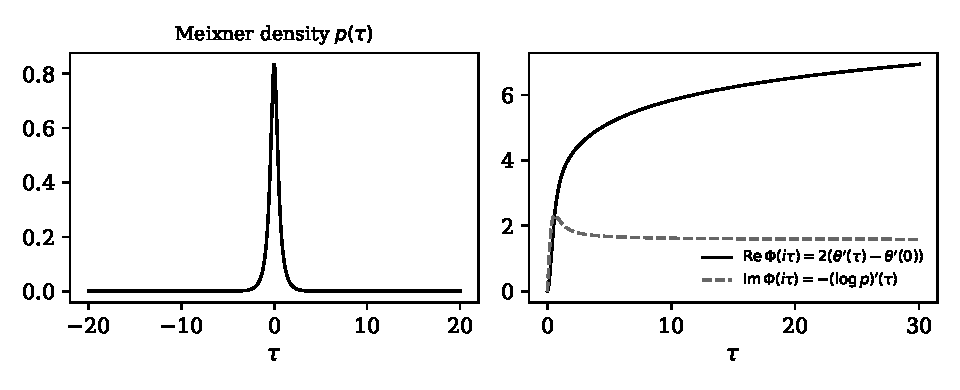
\includegraphics[width=0.95\textwidth]{rzfig/fig_meixner.pdf}
\caption{Left: the Meixner density $p(\tau)\propto|\Gamma(\frac14+\frac{i\tau}2)|^2$. Right: the real and imaginary parts of the Bernstein function $\Phi_\Gamma(i\tau)$ of Proposition~\ref{rz:prop:bernstein}, written $\Phi(i\tau)$ in the legend. The real part is $2(\theta'(\tau)-\theta'(0))$ and grows like $\log\tau$; the imaginary part is the Meixner score $-\frac{d}{d\tau}\log p$ and tends to $\pi/2$, the exponential tail rate of $p$.}
\label{rz:fig:meixner}
\end{figure}

\begin{theorem}\label{rz:thm:gammaggc}
Let $c=-\theta'(0)=\frac12(\log\pi-\psi(\frac14))\approx2.68609$ be the constant of \eqref{rz:eq:c}. Then
\[
\frac{e^{-c\sqs}}{G(s)}=\frac{\Gamma(\frac14)\,\pi^{\sqs/2}\,e^{-c\sqs}}{\Gamma(\frac14+\frac\sqs2)}=\exp\Bigl(-\int_0^\infty\log\Bigl(1+\frac st\Bigr)U_\Gamma(t)\,dt\Bigr),
\]
with
\[
U_\Gamma(t)=\frac{\theta'(\sqrt t)-\theta'(0)}{2\pi\sqrt t}=\frac{1}{2\pi\sqrt t}\sum_{k\ge0}\frac{t}{c_k\,(c_k^2+t)}\ge0 .
\]
So $e^{-c\sqs}/G(s)$ is the Laplace transform of a GGC, and its Thorin distribution function is $(\theta(\sqrt t)-\theta'(0)\sqrt t)/\pi$, a convex increasing function of $\sqrt t$.
\end{theorem}

\begin{proof}
With $f(u)=\Gamma(\frac14+\frac u2)\pi^{-u/2}$ we have $f'(0)/f(0)=\frac12\psi(\frac14)-\frac12\log\pi=\theta'(0)=-c$, and $\frac{d}{du}[\log f(u)-uf'(0)/f(0)]=\frac12\Phi_\Gamma(u)=\frac12\int(1-e^{-uy})\nu(dy)$. Integrating from $0$, $\log f(u)/f(0)-uf'(0)/f(0)=\int(e^{-uy}-1+uy)\frac{\tilde\mu(dy)}{y}$ with $\tilde\mu=\frac12\nu\ge0$. Lemma~\ref{rz:lem:sin2} gives $U_\Gamma(t)=\frac{1}{2\pi\sqrt t}\int2\sin^2(\frac{y\sqrt t}2)\frac12\nu(dy)=\frac{1}{2\pi\sqrt t}\sum_k\int_0^\infty(1-\cos y\sqrt t)e^{-c_ky}dy$, which is the series stated, and Proposition~\ref{rz:prop:bernstein} identifies it with $\theta'$.
\end{proof}

Multiplying $1/G$ by $e^{-c\sqs}$ adds the Thorin density $\frac{c}{2\pi\sqrt t}$, and $U_\Gamma=-U_G+\frac{c}{2\pi\sqrt t}$, which is the identity $c-b=\sum_k(\frac1{c_k}-\frac1{2k+2})$, has no negative part. This is the positive counterpart of Theorem~\ref{rz:thm:gamma}, where the gamma factor appeared as a renormalised product with a signed Thorin density: the archimedean factor becomes positive after one explicit tilt, which leaves the zeros as the only possible source of negativity in the floor of Section~\ref{rz:sec:floor}.

\subsubsection{Meixner Pollaczek polynomials and the local Riemann Hypothesis}

The Meixner law is also the orthogonality measure of the Meixner Pollaczek polynomials, and through them it controls the zeros of the Mellin transforms of the even Hermite functions. Let $\psi_{2m}(x)=H_{2m}(\sqrt{2\pi}\,x)e^{-\pi x^2}$ be the even Hermite functions, eigenfunctions of the Fourier transform $\hat f(y)=\int f(x)e^{-2\pi ixy}dx$ with eigenvalue $(-1)^m$. Define the Mellin transform $\mathcal Mf(s)=\int_0^\infty x^{s-1}f(x)dx$ and $\Gamma_{\R}(s)=\pi^{-s/2}\Gamma(s/2)$. From here to the end of Section~\ref{rz:sec:meixner}, $s$ is the Mellin variable, the argument of $\zeta$, and not the variable of the clock.

\begin{theorem}\label{rz:thm:localRH}
For each $m\ge0$, $Q_m(s)=\mathcal M\psi_{2m}(s)/\Gamma_{\R}(s)$ is a polynomial of degree $m$ satisfying $Q_m(1-s)=(-1)^mQ_m(s)$, and
\[
Q_m(\tfrac12+i\tau)=\kappa_m\,P_m^{(1/4)}\bigl(\tfrac\tau2;\tfrac\pi2\bigr),
\]
where $P_m^{(\lambda)}(x;\phi)$ are the Meixner Pollaczek polynomials and $\kappa_m\ne0$. These are the orthogonal polynomials of the Meixner law $p$. Consequently all zeros of $Q_m$ lie on $\Re s=\frac12$ and are simple: the Mellin transform of every even Hermite function satisfies the Riemann Hypothesis.
\end{theorem}

\begin{proof}
Expanding $H_{2m}(\sqrt{2\pi}\,x)=\sum_jh_jx^{2j}$ gives
\[
\mathcal M\psi_{2m}(s)=\frac12\Gamma_{\R}(s)\sum_jh_j\pi^{-j}(s/2)_j
\]
with Pochhammer symbols, a polynomial of degree $m$ times $\Gamma_{\R}(s)$. Tate's local functional equation \cite[Theorem 2.4.1 and Section 2.5]{Tate67}, $\mathcal Mf(s)/\Gamma_{\R}(s)=\mathcal M\hat f(1-s)/\Gamma_{\R}(1-s)$ for even $f$, applied to the eigenfunction $\psi_{2m}$ gives $Q_m(1-s)=(-1)^mQ_m(s)$, so $i^{-m}Q_m(\frac12+i\tau)$ is a real polynomial $R_m(\tau)$. By Mellin Plancherel,
\[
\int_0^\infty\psi_{2m}\psi_{2n}\,dx=\frac1{2\pi}\int_{\R}Q_m\overline{Q_n}\,|\Gamma_{\R}(\tfrac12+i\tau)|^2d\tau=\sqrt2\,i^{m-n}\int_\R R_m(\tau)R_n(\tau)\,p(\tau)\,d\tau,
\]
since $|\Gamma_{\R}(\frac12+i\tau)|^2=\pi^{-1/2}|\Gamma(\frac14+\frac{i\tau}2)|^2=2^{3/2}\pi\,p(\tau)$. The left side vanishes for $m\ne n$, so $(R_m)$ is the orthogonal polynomial sequence of $p$, which with $x=\tau/2$ is the Meixner Pollaczek family with $\lambda=\frac14$, $\phi=\frac\pi2$ \cite[Section 9.7]{KLS}. Orthogonal polynomials of a measure with infinite support have real simple zeros.
\end{proof}

The conclusion is the archimedean local Riemann Hypothesis of Bump, Choi, Kurlberg and Vaaler \cite{BCKV}, seen through the Meixner law: the squared modulus of the archimedean factor on the line, $|\Gamma_{\R}(\frac12+i\tau)|^2=2^{3/2}\pi\,p(\tau)$, is the orthogonality measure, and orthogonality forces the zeros of these Mellin transforms onto the line. We make no priority claim for this route; Meixner Pollaczek expansions of $\Xi$ in the literature are reviewed in Section~\ref{rz:sec:mpexp}. We checked numerically that the roots of $Q_m$ have real part $\frac12$ to 50 digits for $m\le8$, and that $Q_m(\frac12+i\tau)/P_m^{(1/4)}(\tau/2;\pi/2)$ is constant, with $\kappa_2=-16$, $\kappa_3=-192i$, $\kappa_5=61440i$.

\subsubsection{Zeta in Meixner coordinates}\label{rz:sec:mpexp}

Expansions of $\zeta$ and $\Xi$ in these polynomials have been studied before. Kuznetsov \cite{Kuz2007,Kuz2008} expands $\Xi$ and Dirichlet $L$ functions in Meixner Pollaczek polynomials; Inoue \cite{Inoue} studies the symmetric expansion of the completed zeta function, the multiplicative structure of its coefficients and the zeros of the approximating polynomials; Romik \cite{Romik} expands $\Xi$ itself in the symmetric Meixner Pollaczek basis $P_n^{(3/4)}(x;\frac\pi2)$, together with the Hermite and continuous Hahn bases, and derives coefficient asymptotics; and Candelpergher \cite{Candelpergher} gives related polynomial expansions whose polynomials have their roots on the line. The expansions below first divide $\xi$ by the archimedean factor $\Gamma_{\R}$, or by its modulus, which leads to the parameter $\lambda=\frac14$ of the Meixner law. They are included for comparison with the Thorin picture and are not claimed as new.

The map $\mathcal U f(\tau)=\mathcal Mf(\frac12+i\tau)/\Gamma_{\R}(\frac12+i\tau)$ is, by the Mellin Plancherel identity in the proof of Theorem~\ref{rz:thm:localRH}, a unitary map from $L^2(0,\infty)$ onto $L^2(\sqrt2\,p(\tau)d\tau)$, carrying the even Hermite functions to the Meixner Pollaczek polynomials. Dilations become multipliers, $\mathcal U[f(n\,\cdot)]=n^{-1/2-i\tau}\mathcal Uf$. The function $g(x)=(2\pi^2x^4-3\pi x^2)e^{-\pi x^2}=\frac12(xD)(xD+1)e^{-\pi x^2}$, with $D=d/dx$, has $\mathcal Ug=\frac14s(s-1)$, a Meixner Pollaczek combination of degree two, and its dilation sum $\Omega$ is, up to the factor $\frac12x^{-1/2}$, the P\'olya kernel $\Phi$ of Section~\ref{ch:clock} in the variable $x=e^u$:
\[
\Omega(x)=\sum_{n\ge1}g(nx)=\tfrac12x^{-1/2}\Phi(\log x),\qquad \mathcal U\Omega=\tfrac14s(s-1)\zeta(s)\big|_{s=\frac12+i\tau}.
\]
So in Meixner coordinates $\frac14s(s-1)\zeta(s)$ on the critical line is the image of a function in $L^2(0,\infty)$ and has a convergent Meixner Pollaczek expansion
\[
\tfrac14s(s-1)\zeta(s)=\sum_{m\ge0}a_{2m}\,Q_m(s),\qquad a_{2m}=\frac{\langle\Omega,\psi_{2m}\rangle}{\langle\psi_{2m},\psi_{2m}\rangle},
\]
in $L^2(p)$. Each $Q_m$ satisfies the local Riemann Hypothesis, and $\zeta$ is a superposition of them. We ask whether the property survives in the partial sums.

\begin{table}[htbp]
\centering
\small
\begin{tabular}{rl@{\qquad}rl@{\qquad}rl}
\toprule
$m$ & $a_{2m}$ & $m$ & $a_{2m}$ & $m$ & $a_{2m}$\\
\midrule
0 & $4.265\times10^{-2}$ & 4 & $-1.796\times10^{-5}$ & 8 & $8.904\times10^{-12}$\\
1 & $8.707\times10^{-2}$ & 5 & $2.056\times10^{-7}$ & 12 & $-4.088\times10^{-19}$\\
2 & $1.916\times10^{-2}$ & 6 & $5.080\times10^{-9}$ & 16 & $-3.882\times10^{-26}$\\
3 & $6.391\times10^{-4}$ & 7 & $-3.212\times10^{-10}$ & 24 & $5.961\times10^{-42}$\\
\bottomrule
\end{tabular}
\caption{Meixner Pollaczek coefficients of $\frac14s(s-1)\zeta(s)$, equivalently Hermite coefficients of $\Omega(x)=\sum_{n\ge1}g(nx)=\frac12x^{-1/2}\Phi(\log x)$.}
\label{rz:tab:mp}
\end{table}

The coefficients decay faster than geometrically (Table~\ref{rz:tab:mp}), but the polynomials grow, and the expansion converges slowly as $|\tau|$ grows: at $s=\frac12+5i$ the partial sums with $N=8,16,24$ give $-4.4508$, $-4.4279$, $-4.4291$ for the real part against the exact $-4.4302$, while near the first zero $\frac12+14.1347i$ they are still far from zero at $N=24$. The partial sums $\sum_{m\le N}a_{2m}Q_m(s)$ mix polynomials of both parities under $s\mapsto1-s$, so they have no reason to vanish on the critical line, and for $N=12$ and $N=24$ they do not: all their zeros lie off the line, the nearest to the first zeta zero being $1.92+14.13i$ for $N=12$ and $0.62+14.20i$ for $N=24$. The asymmetric expansion therefore does not test whether the local Riemann Hypothesis survives the superposition; the symmetric expansion does.

The symmetric choice is the real even function $F(\tau)=(\tau^2+\frac14)Z(\tau)$, proportional to $\Xi(\tau)/|\Gamma(\frac14+\frac{i\tau}2)|$, expanded in the even Meixner Pollaczek polynomials $P_{2m}^{(1/4)}(\tau/2;\frac\pi2)$, normalised as in \cite[Section 9.7]{KLS}. Its truncations, the orthogonal projections of $F$ in $L^2(p)$ onto the even polynomials of degree at most $2M$, are real even polynomials, and their real zeros can be compared with the ordinates. The first coefficients are $-0.642$, $-1.117$, $-0.284$, $-0.027$, $0.071$; from $m=3$ on they alternate in sign, and from $m=4$ on their modulus decreases slowly, to about $0.02$ at $m=10$ and $0.01$ at $m=20$. The slow decay reflects the polynomial growth of $F$ against the exponential decay of $p$: the expansion converges in $L^2(p)$, but its truncations approximate $F$ poorly at the ordinates. The truncation of degree $40$ has real zeros at $14.32$, $17.48$, $19.98$, $23.12$, $26.47$, $30.09$, $34.02$, $38.29$ in $[0,40]$, against the ordinates $14.13$, $21.02$, $25.01$, $30.42$, $32.94$, $37.59$. The real zeros of the truncations do not track the ordinates: the zero nearest $14.13$ is $14.50$, $14.32$, $14.16$, $13.73$, $13.54$, $14.84$ for the degrees $38$, $40$, $42$, $50$, $60$, $80$, and there are eight to ten real zeros in $[0,40]$ against six ordinates. Neither expansion suggests a route from the local Riemann Hypothesis to the global one; such a route must use the arithmetic of the full dilation sum, not only the orthogonality of its archimedean pieces.

The factorisation of $\Xi^2$ in Section~\ref{rz:sec:gamma} induces a factorisation of the autocorrelation $\Phi*\Phi$ of the P\'olya kernel, whose Fourier transform is $\Xi^2$. It holds exactly for $|\zeta|^2$ and formally for the Dirichlet series, where the arithmetic factor is a positive measure.

\begin{proposition}\label{rz:prop:autocorr}
The integral $\mathcal C(v)=\int p(\tau)\,|\zeta(\frac12+i\tau)|^2e^{iv\tau}\,d\tau$ converges absolutely, and
\[
(\Phi*\Phi)(v)=2^{-3/2}\Bigl(\frac{d^2}{dv^2}-\frac14\Bigr)^2\mathcal C(v).
\]
Formally $\mathcal C=\sech(\cdot)^{1/2}*\mathcal A$, with
\[
\mathcal A=\sum_{m,n\ge1}\frac{\delta_{\log(m/n)}}{\sqrt{mn}},
\]
where $\sech(v)^{1/2}$ is the characteristic function of the Meixner law and $\mathcal A$, whose Fourier transform is formally $|\zeta(\frac12+i\tau)|^2$, is the autocorrelation of the measure $\sum_nn^{-1/2}\delta_{\log n}$. The measure $\mathcal A$ is positive and positive definite, and the series for $\mathcal C$ diverges: truncated at $m,n\le X$ it equals $X\int\sech(v-r)^{1/2}e^{-|r|/2}\,dr+O(X^{1/2})$. This growth comes from the pole of $\zeta$, and the factor $(\frac{d^2}{dv^2}-\frac14)^2$ does not remove it, since $(\frac{d^2}{dv^2}-\frac14)e^{-|v|/2}=-\delta_0$.
\end{proposition}

\begin{proof}
Since $\Phi$ is even, $\int(\Phi*\Phi)(v)e^{i\tau v}dv=\Xi(\tau)^2=\frac14(\tau^2+\frac14)^2\pi^{-1/2}|\Gamma(\frac14+\frac{i\tau}2)|^2|\zeta(\frac12+i\tau)|^2$, and $\pi^{-1/2}|\Gamma|^2=2^{3/2}\pi\,p$. Fourier inversion divides by $2\pi$, the factor $(\tau^2+\frac14)^2$ becomes $(\frac{d^2}{dv^2}-\frac14)^2$, and the inverse transform of the even function $p|\zeta|^2$ is $\mathcal C/(2\pi)$; the constant is $\frac14\,2^{3/2}\pi/(2\pi)=2^{-3/2}$. The integral $\mathcal C$ converges absolutely because $p(\tau)\sim\pi^{-1/2}|\tau|^{-1/2}e^{-\pi|\tau|/2}$ (Proposition~\ref{rz:prop:meixstruct}) and $\zeta(\frac12+i\tau)$ grows at most polynomially. Formally $|\zeta|^2=|\sum n^{-1/2-i\tau}|^2=\sum_{m,n}(mn)^{-1/2}e^{i\tau\log(m/n)}$, and $\int p(\tau)e^{i\tau(v+r)}d\tau=\sech(v+r)^{1/2}$, which gives $\mathcal C=\sech^{1/2}*\mathcal A$. For the truncation put $D_X(\tau)=\sum_{n\le X}n^{-1/2-i\tau}$; the truncated series is exactly $\int p(\tau)|D_X(\tau)|^2e^{iv\tau}d\tau$. For $|\tau|\le X$, $D_X(\tau)=\zeta(\frac12+i\tau)+X^{1/2-i\tau}/(\frac12-i\tau)+O(X^{-1/2})$ \cite[Theorem 4.11]{Titchmarsh}, and for $|\tau|>X$ the bound $|D_X|^2\le4X$ meets the exponential decay of $p$. Since $\int e^{-|r|/2}e^{i\tau r}\,dr=(\frac14+\tau^2)^{-1}$, the squared pole term contributes $X\int p(\tau)(\frac14+\tau^2)^{-1}e^{iv\tau}d\tau=X\int\sech(v-r)^{1/2}e^{-|r|/2}\,dr$, up to an exponentially small error from $|\tau|>X$; the remaining terms contribute $O(X^{1/2})$ uniformly in $v$, the largest being the cross term of $\zeta$ with the pole term. Finally $(\frac{d^2}{dv^2}-\frac14)^2$ turns $X\int\sech(v-r)^{1/2}e^{-|r|/2}\,dr$ into $-X(\frac{d^2}{dv^2}-\frac14)\sech(v)^{1/2}$, which is not zero.
\end{proof}

So the P\'olya autocorrelation is the Meixner characteristic function smeared over the multiplicative lattice $\{\log(m/n)\}$ with the positive weights $(mn)^{-1/2}$, and then acted on by the pole operator $(\frac{d^2}{dv^2}-\frac14)^2$. Both pieces are positive, the Meixner factor being a GGC transform in $v^2$ and $\mathcal A$ a positive measure, but convolution with a positive measure does not preserve the GGC property, so the GGC structure of the Meixner factor does not pass to the product. The lattice sum also needs a counterterm, the pole term of the approximate functional equation, which comes from the same pole of $\zeta$ that produced the atom at $-\frac14$ in Proposition~\ref{rz:prop:theta}. Problem~\ref{rz:prob:meixner} of Section~\ref{ch:rz4} asks for the regularised form of $\sech(\cdot)^{1/2}*\mathcal A$ and whether it has a Thorin or Lee and Yang structure in $v$.

\subsection{An infinitely divisible floor for the reciprocal Xi function}\label{rz:sec:floor}

Theorem~\ref{rz:thm:gammaggc} makes the archimedean factor positive after one stable tilt. Multiplying $\varphi=RG$ by the GGC transform $e^{-c\sqs}/G$ gives $e^{-c\sqs}R$, which we call the floor of the reciprocal Xi function. In the floor the zeros are the only possible source of negativity, and the floor is a GGC exactly when RH holds. Its infinite divisibility, as proved here, rests on the positivity of $w$, which is proved in Section~\ref{ch:rz3}.

\begin{theorem}\label{rz:thm:floor}
Unconditionally, $e^{-c\sqs}\,\xi(\frac12)/\xi(\frac12+\sqs)$ is the Laplace transform of an infinitely divisible law on $(0,\infty)$ with L\'evy density
\[
\frac{W(x)+c/(2\sqrt{\pi x})}{x},\qquad W(x)=\tfrac12\sum_\rho e^{x(\rho-\frac12)^2},
\]
and $W(x)+c/(2\sqrt{\pi x})>0$ for all $x>0$. The following are equivalent: (i) RH; (ii) this law is a GGC; (iii) $W(x)+c/(2\sqrt{\pi x})$ is completely monotone; (iv) $W$ is completely monotone. The proof uses $w>0$, which is Theorem~\ref{rz:thm:id} of Section~\ref{ch:rz3} and rests on the verification of RH to height $50$, an explicit bound for $N(T)$ \cite{HSW22} and the enclosures E1 to E3.
\end{theorem}

\begin{proof}
$e^{-c\sqs}R=\varphi\cdot(e^{-c\sqs}/G)$ is the product of the transform of an infinitely divisible law (Theorem~\ref{rz:thm:id}) and a GGC (Theorem~\ref{rz:thm:gammaggc}), so it is infinitely divisible, and its L\'evy density is the sum $\{w(x)+\int e^{-xt}U_\Gamma(t)dt\}/x$. By Proposition~\ref{rz:prop:W0erfc} and Theorem~\ref{rz:thm:gammaggc}, $\int e^{-xt}U_\Gamma(t)dt=W_0(x)+\frac{c}{2\sqrt{\pi x}}$, and $w+W_0=W$ by \eqref{rz:eq:weil}. Positivity holds because $w>0$ and $U_\Gamma\ge0$. For the equivalences: GGC means the L\'evy density times $x$ is completely monotone, so (ii)$\Leftrightarrow$(iii). Under RH $W=\sum e^{-x\gamma^2}$ is completely monotone, so (i)$\Rightarrow$(iv)$\Rightarrow$(iii). If (ii) holds, the transform is analytic on $\cut$ and agrees with $e^{-c\sqs}R$ on $(0,\infty)$, so by uniqueness of analytic continuation $R$ has no poles in $\cut$; since $R$ has no zeros and $G$ is analytic and zero free on $\cut$, $\varphi=RG$ is analytic and zero free there, and Proposition~\ref{rz:prop:rh} gives RH.
\end{proof}

Infinite divisibility alone is not new: by Theorem~\ref{thm:ch12:idsd} \cite[Theorem A]{P26}, $W>0$ and $W'<0$ on $(0,\infty)$, so $R$ itself is infinitely divisible and self decomposable, and so is its product with the stable factor $e^{-c\sqs}$; Section~\ref{ch:sato} draws the consequences of self decomposability. What the floor adds is the splitting of its canonical function $k=W+c/(2\sqrt{\pi x})$ as $k=w+\int e^{-xt}U_\Gamma(t)\,dt$, an arithmetic part plus a completely monotone archimedean part contributed by the Meixner law (Theorem~\ref{rz:thm:gammaggc}). The tilt, with the constant $c=\zeta'(\frac12)/\zeta(\frac12)$, removes the negative part of the Thorin density of $1/G$, which lies at $t<\tau_0^2$; in the L\'evy picture it cancels the negative tail of $W_0$, since $W_0+c/(2\sqrt{\pi x})=\int e^{-xt}U_\Gamma(t)\,dt>0$. In law the floor adds to $X_R$ an independent first passage time $L_c$ of $\sqrt2B$ to the level $c$. At the basepoints $\alpha>\frac12$ the clocks are the centre clock tilted and subordinated by a drift and a stable one half process (Section~\ref{ch:bphit}), and at the basepoint one the stable factor $e^{-b_1\sqs}$, with $b_1=\sum_\rho\rho^{-1}$, plays the role of the tilt (Section~\ref{ch:basepoint}). Everything that could fail therefore lies in $w$, and RH is the upgrade of $k$ from positivity, the lowest rung of the ladder of Section~\ref{ch:heat}, to complete monotonicity, its top.

\subsubsection{The sine squared lemma at the floor}

Theorem~\ref{rz:thm:floor} describes the floor through its L\'evy density in the variable $s$. The sine squared lemma works one level earlier, with the primal L\'evy measure in the variable $u=\sqs$. To apply it to the floor we identify the primal function and its L\'evy measure, and then follow the two stages of the proof of Lemma~\ref{rz:lem:sin2}: a subordination stage that produces the L\'evy density in $s$, and a Bernstein stage that produces the Thorin measure. As in that proof, from here to the end of the section $x$ is the variable of the primal L\'evy measure, and the time of the heat trace is written $y$.

The floor is $e^{-c\sqs}R(s)=f(0)/f(\sqs)$ with primal function $f(u)=e^{cu}\xi(\frac12+u)$, and $f'(0)/f(0)=c$ because $\xi'(\frac12)=0$. The tilt contributes the linear term $cu$ to $\log f$, which cancels in $\log f(u)/f(0)-uf'(0)/f(0)=\log\xi(\frac12+u)/\xi(\frac12)$, so the primal L\'evy measure of the floor is that of $\xi$ at the centre. Collecting the three factors of $\xi(\frac12+u)=\frac12(u^2-\frac14)\,\pi^{-1/4}f_\Gamma(u)\,\zeta(\frac12+u)$, where $f_\Gamma(u)=\pi^{-u/2}\Gamma(\frac14+\frac u2)$, gives formally
\begin{equation}\label{rz:eq:primalxi}
\tilde\mu_\xi(dx)=-2\cosh\bigl(\tfrac x2\bigr)\,dx+\sum_{k\ge0}e^{-c_kx}\,dx+\sum_{n\ge2}\frac{\Lambda(n)}{\sqrt n}\,\delta_{\log n}(dx).
\end{equation}
The first term comes from $u^2-\frac14=(u+\frac12)(u-\frac12)$, each linear factor $1+u/a$ contributing $-e^{-ax}dx$ by Frullani (with $a=-\frac12$ by continuation); the second is $\frac12\nu$ (Proposition~\ref{rz:prop:bernstein} and the proof of Theorem~\ref{rz:thm:gammaggc}); the third is the prime measure of Proposition~\ref{rz:prop:zetaright} at $\beta=\frac12$. By the explicit formula, as distributions on $x>0$,
\begin{equation}\label{rz:eq:primalzeros}
\tilde\mu_\xi(dx)=-\sum_\rho e^{(\rho-\frac12)x}\,dx,\qquad\text{which under RH is}\qquad-2\sum_{\gamma>0}\cos(\gamma x)\,dx .
\end{equation}

\begin{proposition}\label{rz:prop:twostage}
Apply the two stages of Lemma~\ref{rz:lem:sin2} to $\tilde\mu_\xi$, regularising $\int_0^\infty\cos(\gamma x)dx=0$ and the growing term of \eqref{rz:eq:primalxi} by analytic continuation.
\begin{enumerate}
\item[(i)] Subordination stage: $(4\pi y)^{-1/2}\int_0^\infty(1-e^{-x^2/4y})\,\tilde\mu_\xi(dx)=W(y)$, the heat trace over the zeros. With the tilt, the canonical function of the floor is $k(y)=W(y)+c/(2\sqrt{\pi y})$, as in Theorem~\ref{rz:thm:floor}, and its positivity is proved.
\item[(ii)] Bernstein stage: $U(t)=\frac{1}{2\pi\sqrt t}\int_0^\infty2\sin^2(\frac{x\sqrt t}2)\,\tilde\mu_\xi(dx)$ equals $\sum_{\gamma>0}\delta_{\gamma^2}$ under RH, and the Thorin measure of the floor is $U+\frac{c}{2\pi\sqrt t}dt$.
\end{enumerate}
The two stages are linked by $W(y)=\int_0^\infty e^{-yt}U(t)\,dt$. The floor is a GGC exactly when $U+\frac{c}{2\pi\sqrt t}\,dt\ge0$, that is, when $k$ is completely monotone; by Theorem~\ref{rz:thm:floor} this happens exactly under RH, and then $U=\sum_{\gamma>0}\delta_{\gamma^2}\ge0$.
\end{proposition}

\begin{proof}
(i) For $\tilde\mu=-2\cos(\gamma x)dx$,
\[
\int_0^\infty(1-e^{-x^2/4y})(-2\cos\gamma x)\,dx=2\int_0^\infty e^{-x^2/4y}\cos\gamma x\,dx=\sqrt{4\pi y}\,e^{-\gamma^2y}.
\]
Without RH the same computation with $e^{(\rho-\frac12)x}$ gives $e^{y(\rho-\frac12)^2}$, so the result is $W$ in general. (ii) $\int_0^\infty(1-\cos x\sqrt t)(-2\cos\gamma x)\,dx=\pi\,\delta(\sqrt t-\gamma)$, and $\frac{1}{2\pi\sqrt t}\pi\,\delta(\sqrt t-\gamma)=\delta(t-\gamma^2)$. The link is the identity $(1-e^{-x^2/4y})/\sqrt y=\int_0^\infty e^{-yt}\{1-\cos x\sqrt t\}\frac{dt}{\sqrt{\pi t}}$ used in the proof of Lemma~\ref{rz:lem:sin2}.
\end{proof}

The lemma preserves positivity, so if $\tilde\mu_\xi$ were a positive L\'evy measure the floor would be a GGC and RH would follow. But $\tilde\mu_\xi$ is not positive. Its pole part $-2\cosh(x/2)\,dx$ is negative, and at large $x$ it cancels the mean density $e^{x/2}dx$ of the prime atoms, leaving the oscillating sum over zeros \eqref{rz:eq:primalzeros}. Its pieces are not admissible either: the pole part grows like $e^{x/2}$ and the prime part has infinite mass, so the hypothesis of Lemma~\ref{rz:lem:sin2} fails and both stages need regularisation. The positive pieces are those already used: the gamma part, which gives Theorem~\ref{rz:thm:gammaggc}, and the prime part, which gives Proposition~\ref{rz:prop:zetaright} once it is moved to the right of $\Re z=1$. At the centre the lemma turns the question into one about a signed input whose sine squared image is positive if and only if RH holds.

\subsubsection{Complete monotonicity to finite order}

Positivity at stage (i) of Proposition~\ref{rz:prop:twostage} is Theorem~\ref{rz:thm:floor}; positivity at stage (ii) is complete monotonicity of $k(y)=W(y)+c/(2\sqrt{\pi y})$, that is $(-1)^nk^{(n)}\ge0$ for every $n$. Between the two lie the same inequalities for finitely many $n$, and the two range argument of Theorem~\ref{rz:thm:id} proves them for every order up to $10^{10}$.

\begin{theorem}\label{rz:thm:nmono}
Let $k(y)=W(y)+c/(2\sqrt{\pi y})$. For every $n\le10^{10}$ and every $y>0$,
\[
(-1)^n\,k^{(n)}(y)>0 .
\]
Consequently, by Williamson's theorem, for each $1\le n\le10^{10}$ there is a positive measure $\Omega_n$ on $(0,\infty)$ with $k(y)=\int(1-ty)_+^{\,n-1}\,\Omega_n(dt)$. For $n\ge1$ the proof uses the verification of RH to height $T_0=3\times10^{12}$ \cite{PT21}, an explicit bound for $N(T)$ \cite{HSW22} and one interval enclosure (E4, Section~\ref{rz:sec:num}), and no other information about zeros.
\end{theorem}

\begin{proof}
The case $n=0$ is the positivity in Theorem~\ref{rz:thm:floor}. Fix $1\le n\le10^{10}$ and put $y_n=0.05/n$.

Small $y$. Write $k=w+(W_0+\frac{c}{2\sqrt{\pi y}})$. By Theorem~\ref{rz:thm:gammaggc} the bracket is $\int e^{-ty}U_\Gamma(t)\,dt$ with $U_\Gamma\ge0$, so $(-1)^n$ times its $n$th derivative is $L_n(y)=\int t^ne^{-ty}U_\Gamma(t)dt$, decreasing in $y$. Since $\theta'(\tau)-\theta'(0)\ge\frac{2\tau^2}{\frac14+\tau^2}\ge1$ for $\tau\ge\frac12$ (the $k=0$ term of the series in Theorem~\ref{rz:thm:gammaggc}),
\[
L_n(y)=\frac1\pi\int_0^\infty\tau^{2n}e^{-y\tau^2}\bigl(\theta'(\tau)-\theta'(0)\bigr)d\tau\ge\frac{\Gamma(n+\frac12)}{2\pi}\,y^{-n-\frac12}-\frac{2^{-2n-1}}{\pi(2n+1)} .
\]
On the other side $(-1)^nw^{(n)}=(-1)^n4^{-n}e^{y/4}-(-1)^nP^{(n)}$. $P$ is analytic in $\Re y>0$, and on the circle $|z-y|=y/2$ one has $|z|\ge y/2$ and $\Re(1/z)\ge2/(3y)$, so Cauchy's estimate gives
\begin{align*}
|P^{(n)}(y)|&\le n!\,(2/y)^n\,(2\pi y)^{-1/2}\sum_m\Lambda(m)m^{-1/2}e^{-(\log m)^2/6y}\\
&\le C_0\,n!\,(2/y)^n\,(2\pi y)^{-1/2}e^{-(\log2)^2/6y},
\end{align*}
where $C_0=0.54993$ bounds $e^{(\log2)^2/6y}\sum_m\Lambda(m)m^{-1/2}e^{-(\log m)^2/6y}$ for every $y\le0.05$, each term being increasing in $y$ (enclosure E4). Divide by the leading term of the lower bound for $L_n$ and use Gautschi's inequality $n!/\Gamma(n+\frac12)<\sqrt{n+1}$ \cite[(5.6.4)]{DLMF}. For $y\le y_n$ we have $(\log2)^2/6y\ge1.6015\,n$, so the ratio is at most
\[
r_n=C_0\sqrt{2\pi}\sqrt{n+1}\,e^{(\log2-1.6015)n},
\]
which decreases in $n$, since $r_{n+1}/r_n\le\sqrt{3/2}\,e^{\log2-1.6015}<\frac12$, and satisfies $r_n\le r_1<0.786$ (enclosure E4). Hence, for $y\le y_n$,
\[
(-1)^nk^{(n)}(y)\ge(1-r_n)\frac{\Gamma(n+\frac12)}{2\pi}y_n^{-n-\frac12}-\frac{2^{-2n-1}}{\pi(2n+1)}-4^{-n}e^{y/4}.
\]
The first term is at least $0.214\,\Gamma(\frac32)\,20^{3/2}/(2\pi)>2.6$, since $\Gamma(n+\frac12)(20n)^{n+\frac12}$ increases in $n$, and the two negative terms total less than $0.27$. So $(-1)^nk^{(n)}>0$ on $(0,y_n]$ for every $n\ge1$.

Large $y$. Here $(-1)^nk^{(n)}=(-1)^nW^{(n)}+\frac{c\,\Gamma(n+\frac12)}{2\pi}y^{-n-\frac12}$. Zeros with $0<\gamma\le T_0$ lie on the line and contribute $\gamma^{2n}e^{-y\gamma^2}>0$. Any other zero has $\gamma>T_0$ and contributes at most $(\gamma+1)^{2n}e^{-y(\gamma^2-\frac14)}$ in modulus. Let $y\ge y_n$. Since $n/y\le20n^2<T_0^2$, the function $(\gamma+1)^{2n}e^{-y\gamma^2}$ decreases for $\gamma\ge T_0$, so by $N(t+1)-N(t)\le2\log(t+1)$, which follows from \cite{HSW22} as in the proof of Theorem~\ref{rz:thm:id}, the zeros with $T_0+j<\gamma\le T_0+j+1$ contribute at most $b_j=2\log(T_0+j+1)\,(T_0+j+1)^{2n}e^{-y((T_0+j)^2-\frac14)}$. For $n\le10^{10}$ we have $b_{j+1}/b_j\le\exp\bigl(\frac{2n}{T_0}+\frac{1}{T_0\log T_0}-\frac{2T_0+1}{20n}\bigr)<10^{-13}$, so the tail is at most $2b_0=4\log(T_0+1)\,(T_0+1)^{2n}e^{-y(T_0^2-\frac14)}$. Its ratio to the positive term $\frac{c\,\Gamma(n+\frac12)}{2\pi}y^{-n-\frac12}$ is a constant multiple of $y^{n+\frac12}e^{-y(T_0^2-\frac14)}$, which decreases for $y\ge y_n$ because $T_0^2-\frac14>20n(n+\frac12)$. At $y=y_n$, using $\Gamma(n+\frac12)\ge\Gamma(\frac32)$ and $y_n<1$, the logarithm of the ratio is at most
\[
\log\frac{8\pi\log(T_0+1)}{c\,\Gamma(\frac32)}+2n\log(T_0+1)-\frac{T_0^2-\frac14}{20n}<-4.4\times10^{13},
\]
because the left side increases with $n$, and at $n=10^{10}$ its first term is below $6$ while $y_n(T_0^2-\frac14)\approx4.5\times10^{13}$ exceeds $2n\log(T_0+1)<5.8\times10^{11}$ by a wide margin. So the tail is smaller than the positive term.

Williamson's theorem \cite{Williamson} characterises $n$ monotone functions on $(0,\infty)$ as mixtures of $(1-ty)_+^{n-1}$ with positive weights; since $k(\infty)=0$, this gives $\Omega_n$.
\end{proof}

The small $y$ branch works for every $n$, but only on $(0,0.05/n]$, the range forced by the Cauchy estimate. The large $y$ branch must cover the rest, and there the bound of the proof lets the positive term $c\,\Gamma(n+\frac12)y^{-n-\frac12}/(2\pi)$ contributed by the tilt dominate the zeros above $T_0$ whenever $y_n(T_0^2-\frac14)>2n\log(T_0+1)+6$. This sufficient condition holds while $n<8.8\times10^{10}$, and we state the safe round number $10^{10}$. By Theorem~\ref{rz:thm:floor}, RH is equivalent to the inequality for every $n$, and Bernstein's theorem is the limit of Williamson's as $n\to\infty$.

Theorem~\ref{rz:thm:nmono} is the analogue for the floor of the derivative ladder that Section~\ref{ch:heat} climbs for the clock. It is a consequence of the verification of RH to height $T_0$ and carries no information about the zeros beyond it: an off line zero above $T_0$ is invisible to derivatives of order below about $yT_0^2$, the order at which the peak of $\gamma^{2n}e^{-y\gamma^2}$ passes $T_0$, and could break complete monotonicity only beyond that order. With the Cauchy estimate of the proof, the reachable order grows roughly linearly with $T_0$, and sharper estimates reach further. Theorem~\ref{thm:ch12:cm} \cite[Theorem 7.10]{P17} proves $(-1)^nW^{(n)}>0$ for every $n\le10^{17}$, and the same range follows for $k$ because $c/(2\sqrt{\pi y})$ is completely monotone. The reach of its proof grows like the square of the verified height up to a logarithm (Section~\ref{sec:ch12:reach}): at $y=1/20000$, where the proof passes from the primes to the zeros, it reaches orders up to about $yH^2/\log(H^2/\gamma_0^2)$, with $H=10^{12}$ the verified height that proof uses and $\gamma_0\in(20,50]$ the height of the low zero that dominates, a factor $\log(H^2/\gamma_0^2)\approx48$ below the order $yH^2$ at which an off line zero above $H$ becomes visible. Theorem~\ref{thm:ch12:window} closes that gap with a dominating zero that follows the peak of $\gamma^{2n}e^{-y\gamma^2}$: it proves the signs for every $n\le y(H-23)^2$ at every $y\ge1.29$, with $H=3\times10^{12}$, and, with Theorem~\ref{thm:ch12:cmint}, for every $n\le1.16\times10^{25}$ at every $y>0$, for $W$ and so for $k$. In every version the reach is set by the verified height and lies below that order: the Thorin measure of the floor is certified positive up to a resolution that grows with the verified height, and RH is the statement that it stays positive at infinite resolution, which no finite number of rungs reaches.

In the floor the archimedean factor supplies the completely monotone part of $k$ but none of the arithmetic: the jumps of $N$, the negative excursions of $S$, and the cancellation that must make $W$ completely monotone. The arithmetic inputs of this section are the verified zeros used in Theorem~\ref{rz:thm:nmono} and the positivity of $w$, used in Theorem~\ref{rz:thm:floor} and proved in Section~\ref{ch:rz3}.
